%% =====================================================================
%% BiTeM at the TRECVID 2026 VQA Task (Task 1 AG, Task 2 MC)
%%
%% Template: main_knafou_ntcir.pdf (BITEM at NTCIR-19 R2C2), acmart sigconf,
%% matching repos/trec-rag/paper/tex/main_bitem_trec_rag.tex.
%% [nonacm] is set because TRECVID proceedings are published by NIST, not ACM.
%%
%% EVERY development number below was re-derived from disk on 2026-09-15 unless
%% a comment says otherwise; the comment adjacent to each claim names the file or
%% command. Official 2026 scores (released to teams 2026-09-28) come from
%% submissions/vqa2026/official_results/, whose PROVENANCE.md records the source.
%% =====================================================================
\documentclass[sigconf,nonacm]{acmart}

\usepackage{booktabs}
\usepackage{array}
\usepackage[htt]{hyphenat}   %% allow hyphenation inside \texttt

%% Breakable literal: paths, model ids and flags are long and unbreakable in a
%% two-column layout, so they overflow into the other column. \lit{} lets them
%% break after the separators that appear in them.
%% Long literals (paths, model ids, flags) overflow a two-column measure.
%% hyphenat's [htt] lets \texttt break; \allowbreak hints are added by hand to
%% the one path long enough to need them.
\newcommand{\run}[1]{\mbox{\textbf{#1}}}   %% run tags: bold, never hyphenated
\newcommand{\lit}[1]{\texttt{#1}}
\sloppy
\emergencystretch=2em
\usepackage{multirow}

%% Numbered citations, as in the NTCIR template this paper follows.
\citestyle{acmnumeric}

\settopmatter{printacmref=false}
\renewcommand\footnotetextcopyrightpermission[1]{}
\pagestyle{plain}

%% Tighter float spacing: this paper carries six tables in ten pages.
\setlength{\textfloatsep}{8pt plus 2pt minus 2pt}
\setlength{\floatsep}{8pt plus 2pt minus 2pt}
\setlength{\intextsep}{8pt plus 2pt minus 2pt}
\setlength{\abovecaptionskip}{4pt}
\setlength{\belowcaptionskip}{2pt}

%% The bibliography is 45 entries in a short paper; set it a size down so the
%% reference list does not outweigh the body.
\renewcommand{\bibfont}{\scriptsize}
\AtBeginDocument{\renewcommand{\bibfont}{\scriptsize}}

%% A marked gap. Used for every quantity that is not yet measurable from disk.
%% A visible gap is correct here; a plausible-looking number would not be.
\newcommand{\gap}[1]{\textsf{\small[#1]}}

\begin{document}

\title{BiTeM at TRECVID 2026 VQA: What a 500-Item Development Set Could Not See}

\author{Esteban Gaillac, Julien Knafou, Paul Van Rijen, Alexandre Flament, Patrick Ruch}
\affiliation{\institution{HES-SO, Geneva, Switzerland}\country{}}
\affiliation{\institution{SIB Swiss Institute of Bioinformatics, Geneva, Switzerland}\country{}}
\email{esteban.gaillac@hesge.ch}

\renewcommand{\shortauthors}{Gaillac et al.}

%% ==================== abstract
\begin{abstract}
We entered both TRECVID 2026 VQA tasks with one locally hosted, open-weight
pipeline built on Qwen3-VL and Qwen3.5, and placed 7th of 15 teams on answer
generation and 10th of 13 on multiple choice. Our development set could not rank
our own runs: the multiple-choice run we nominated as primary finished fourth of
our five, while the 122B run, entered for diversity, and a fusion run we nearly left out
finished first and second, 3.5 and 3.1 points higher. Four identical runs on our 497 development items spread over 4
points, and the 3.5-point effect we missed needs about 900 items to be detected
reliably. We also audit the 2025 collection, our development data. Its multiple-choice gold
is the free-text reference copied verbatim, a few golds are non-answers or
unreachable, and the longest option is correct on 47\,\% of its four-option
questions against 25\,\% chance (41\,\% against 15\,\% on the 2026 labels). Finally, the official answer-generation measures disagree: the same run
ranks 14th, 20th and 41st of 44 depending on the measure, and a slate of one real
answer and nine nonsense strings outscores every official run on METEOR NDCG@10.
\end{abstract}

\keywords{video question answering, multiple choice, benchmark artifacts,
run-to-run variance, evaluation measures}

\maketitle
\pagestyle{empty}   %% no running heads or folios, as in Knafou et al., arXiv:2609.37993v2
\thispagestyle{empty}

\section*{Team Name}
BiTeM

\section*{Subtasks}
Task 1: Answer Generation (AG) \\
Task 2: Multiple Choice (MC)

\section*{Structured Abstract}

\paragraph{Task 1, Answer Generation.}
\emph{Training data.} None: no model was trained or fine-tuned. Pretrained
Qwen3-VL-8B answers from a pool of 16 frames per video. The released 2025 VQA
collection~\cite{awad2025vqa} served as development data and as the source of
the few-shot examples. Speech is transcribed with faster-whisper large-v3-turbo,
and candidate answers are clustered with all-MiniLM-L6-v2 sentence embeddings.

\emph{Runs.}
\begin{itemize}\setlength{\itemsep}{1pt}
\item \texttt{BiTeM\_cons8b\_s8}: eight independent samples of a single short
answer, each on a random 8 of the 16 frames, clustered and ranked by how often
an answer recurs.
\item \texttt{BiTeM\_cons8b\_s16}: the same with 16 samples; our flagship.
\item \texttt{BiTeM\_fewshot8b}: eight samples, plus the four nearest 2025
(question, reference) pairs as examples.
\item \texttt{BiTeM\_all8b}: as \texttt{fewshot8b}, plus a speech transcript for
questions a lexical router flags as verbal.
\item \texttt{BiTeM\_v3control}: our earlier prompt format, one call for ten
increasingly speculative answers, entered as a control.
\end{itemize}

\emph{Significant differences.} The four sampling runs span 0.005 STS@1. The
control is last of our five on STS@1, 0.023 below the next run, but first on
METEOR@1 (0.036 above the next) and on METEOR NDCG@10 (0.077 above the next).

\emph{Component contributions.} Asking for one short answer many times, instead
of ten ranked answers in one call, gained 0.07 STS on development topics and
cost METEOR. Doubling the samples, adding examples and adding routed transcripts
each moved official STS@1 by 0.005 or less.

\emph{Lessons.} The official measures disagree about which of our runs is best.
After submission, minimum-Bayes-risk selection over 16 to 128 samples improved
only the measure it used as its utility (Figure~\ref{fig:mbr}).

\paragraph{Task 2, Multiple Choice.}
\emph{Training data.} None: nothing was trained or fine-tuned. Pretrained
Qwen3-VL-8B, 30B-A3B and 32B, and Qwen3.5-122B, all served by Ollama. Development
used 497 eight-option items built from the 2025 collection~\cite{awad2025vqa}.
Transcripts are produced as in Task~1, for routed questions only.

\emph{Runs} (short names as in Table~\ref{tab:runs}).
\begin{itemize}\setlength{\itemsep}{1pt}
\item \texttt{BiTeM\_mc32b} (\texttt{mc\_32b\_prod}): Qwen3-VL-32B ranks every
option from the frame pool, with a transcript when routed; nominated primary.
\item \texttt{BiTeM\_mc30b} (\texttt{mc\_30b\_prod}): the same with
Qwen3-VL-30B-A3B.
\item \texttt{BiTeM\_mc122b} (\texttt{mc\_122b\_prod}): the same with
Qwen3.5-122B.
\item \texttt{BiTeM\_mc32bdense} (\texttt{mc\_32b\_dense}): \texttt{mc32b} with
32--64 frames for videos longer than 40\,s.
\item \texttt{BiTeM\_mcfusion} (\texttt{mc\_fusion}): reciprocal-rank fusion of the
32B, 122B and 30B option rankings.
\end{itemize}

\emph{Significant differences}, by exact McNemar test against \texttt{mc32b}:
\texttt{mc122b} $+3.5$ points and \texttt{mcfusion} $+3.1$, both at
$p<10^{-5}$ and level with each other ($p=0.46$); \texttt{mc32bdense} $+0.1$
($p=0.89$); \texttt{mc30b} $-1.5$ ($p=0.051$).

\emph{Component contributions.} The choice of model and the three-model fusion
each gained about 3 points. Denser frames on long clips gained nothing
measurable.

\emph{Lessons.} Our 497 development items could not detect 3-point differences,
and we read that as evidence of no difference. The released options carry a
length artifact as strong in 2026 as in 2025. A cascade that escalates likely 8B
errors to 32B was built and withheld: it agreed with \texttt{mc32b} on 96\,\% of
top-1 answers and cost more per question than running 32B everywhere.

%% ==================== intro
\section{Introduction}

The TRECVID Video Question Answering track~\cite{awad2025vqa} asks systems to
answer natural-language questions about short videos. Task~1, Answer Generation
(AG), takes ten distinct ranked free-text answers per question. Task~2, Multiple
Choice (MC), takes a ranking of the released options, scored by exact string
match against one correct option.

Our system is standard: an open-weight video-language model sampled on random
subsets of a video's frames, with answers aggregated across samples and a speech
transcript added when a question seems to need one. Everything runs locally, and
no commercial API is called. Our best runs placed 7th of 15 teams on Task~1 and
10th of 13 on Task~2.

Most of what we learned this year is about evaluation: how small a difference
500 items can detect, and what this task's labels and measures reward. Our
development set could not rank our own Task~2 runs. The run we nominated as primary finished fourth of our five, while the 122B run,
entered for diversity, and a fusion run we nearly left out finished first and
second. Our contributions are:
\begin{itemize}
\item a replicate study of what 497 development items can resolve: four runs of
one configuration spread over 4 points, a fifth of the items flip between runs,
and two 3-point effects we dismissed on this set were real on the 2,428 official
questions;
\item an audit of the MC labels: the gold option is the AG reference copied
verbatim, six golds are non-answers, four cannot be matched by any run, and the
longest option is correct far above chance in both years;
\item evidence that the official AG measures disagree and can be gamed: one run
ranks from 14th to 41st of 44 depending on the measure, a selection rule improves
only the measure it optimises, and one answer padded with nine nonsense strings
tops every official run on METEOR NDCG@10;
\item a list of issues for the organisers, each with a fix
(Table~\ref{tab:organisers}).
\end{itemize}

%% ==================== related
\section{Related Work}

\paragraph{Partial-input baselines and option length.}
Benchmarks can often be solved without their input. Gururangan et
al.~\cite{gururangan2018artifacts} and Poliak et
al.~\cite{poliak2018hypothesisonly} showed this for NLI, and Kaushik and
Lipton~\cite{kaushik2018howmuch} and Sugawara et al.~\cite{sugawara2018easier}
for reading comprehension. For multiple choice, showing only the options beats
the majority baseline in 11 of 12 datasets~\cite{balepur2024artifacts}. Our
longest-option baseline reads neither the video nor the question. The length cue
is known in educational testing: Millman et al.~\cite{millman1965testwiseness}
described test-wiseness, and Haladyna et al.'s item-writing
guidelines~\cite{haladyna2002guidelines} ask for options of about equal length.
ReClor~\cite{yu2020reclor} used such biases to split its test set into easy and
hard halves.

\paragraph{How benchmarks acquire artifacts.}
Adversarial filtering~\cite{zellers2018swag, lebras2020aflite} and balanced
construction~\cite{goyal2017vqav2} are the usual remedies. Aroyo and
Welty~\cite{aroyo2015truth} made explicit the assumptions behind single-annotator
gold, Pavlick and Kwiatkowski~\cite{pavlick2019disagreements} showed that
annotator disagreement does not average out, and Northcutt et
al.~\cite{northcutt2021labelerrors} measured what label errors cost downstream.

\paragraph{Video QA and single-frame bias.}
About half of MovieQA can be answered without the video~\cite{jasani2019movieqa}.
TVQA~\cite{lei2018tvqa} and NExT-QA~\cite{xiao2021nextqa} target temporal and
causal reasoning, while Buch et al.~\cite{buch2022revisiting} and Lei et
al.~\cite{lei2023singleframe} found that much of video QA needs little temporal
information. Video-MME~\cite{fu2025videomme} made duration an explicit axis,
which matters here because a fifth of the 2026 questions come from clips longer
than 40 seconds.

\paragraph{Variance and power.}
Random seeds alone produce differences significant at
$p<10^{-4}$~\cite{reimers2017distributions}, typical NLP experiments are
underpowered~\cite{card2020littlepower}, and LLM results move with prompt
format~\cite{sclar2024formatting} and option order~\cite{zheng2024notrobust}. We
compare paired runs with the exact McNemar test~\cite{mcnemar1947}, which
Dietterich~\cite{dietterich1998approximate} recommends for algorithms run once.

\paragraph{Abstention and cascades.}
Classification with a reject option goes back to Chow~\cite{chow1970reject}, and
selective classification for deep networks to Geifman and
El-Yaniv~\cite{geifman2017selective}. SQuAD~2.0~\cite{rajpurkar2018squad2} made
abstention part of a QA task, Kadavath et al.~\cite{kadavath2022know} asked models
whether they know the answer, and Wen et al.~\cite{wen2025abstention} survey the
area. Like Kamath et al.~\cite{kamath2020selective}, we train a separate error
predictor. Post-abstention~\cite{varshney2023postabstention},
cascades~\cite{chen2023frugalgpt} and self-consistency~\cite{wang2023selfconsistency}
are the closest designs. RFC~4180~\cite{rfc4180} specifies the CSV quoting whose
violation made four golds unreachable.

%% ==================== methods
\section{Methods}
\label{sec:methods}

\subsection{Tasks and data}
\label{sec:data}

\paragraph{Scoring.}
Task~1 is scored with STS, METEOR and BERTScore F1. Before submission we took the
score to be each measure's mean over the ten answers, as in the 2025 scorer. The
2026 report gives, for each measure, the best answer and the mean answer within
the top 1, 5 and 10 and an NDCG computed within the slate, and its summary uses
the three @1 scores and the three NDCG@10. Task~2 is scored by top-1 accuracy and
MRR under exact string matching, so a re-typed or trimmed option counts as wrong.

\paragraph{The 2026 collection.}
Both tasks share 2,443 questions over 1,956 videos. In Task~2, 1,971 questions
have eight options and 472 have four, for a chance rate of 14.9\,\%. The MC file
was released twice, and 2,435 of its option lists changed between the two
versions, so we rebuilt every run against the second. Video durations are
bimodal: the median is 10 seconds, but 212 clips last longer than 40 seconds (up
to 389) and carry 479 questions, a fifth of the task. No development video is
longer than 30 seconds.

\paragraph{Development data.}
The 2025 test collection~\cite{awad2025vqa} was released with its ground truth,
the same file the public scorer uses, so the 2025 evaluation can be reproduced
exactly. We use its 1,978 scoreable questions: 18 have no video and 4 have an
unreachable gold (Section~\ref{sec:benchmark}). For Task~2 we first used the
first 300 questions of the file. That slice turned out to be the most
8B-favouring window of its size in the whole collection, so we replaced it with
497 questions sampled to the 2026 mix of question types and padded from four to
eight options with length-matched distractors from other questions. This set
ranks systems against each other but does not predict 2026 accuracy: its options
are less alike than those of the real eight-option items (mean token overlap
0.07 against 0.18).

\subsection{System}
\label{sec:system}

Both systems use a pool of 16 evenly spaced frames per video, an optional speech
transcript, and a model served locally by Ollama: Qwen3-VL at 8B, 30B-A3B or
32B, or Qwen3.5-122B. Nothing was trained or fine-tuned. Figure~\ref{fig:pipeline}
shows the two pipelines, and Figure~\ref{fig:example} follows one question
through the first.

\begin{figure*}[t]
%% source: paper/figures/figs_method.py; drawn at final size, included unscaled (no text below 9 pt).
\centering
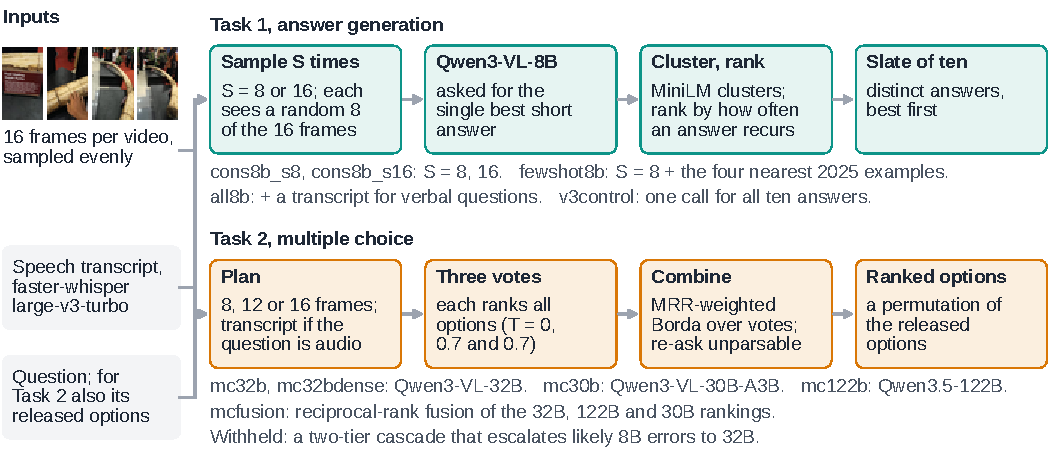
\includegraphics{figures/fig_pipeline.pdf}
\caption{The two pipelines. Both tasks share one pool of 16 evenly spaced frames
per video, an optional speech transcript and a locally served model. Task~1 asks
for one short answer $S$ times, each time on a random 8 of the 16 frames, and
keeps what recurs; Task~2 casts three votes that each rank every option, and
combines them. The notes under each lane name the variant behind each submitted
run.}
\label{fig:pipeline}
\end{figure*}

\paragraph{Task~1.}
We sample $S$ answers ($S=8$ or 16), each from its own random 8 of the 16 frames,
with a prompt that asks for a single short answer in the style of the
references: one clause, no hedging, a pronoun for a single person, number words
for counts. Two additions are optional: a transcript, for questions a lexical
router flags as verbal, and the four most similar 2025 (question, reference)
pairs as examples. Answers are clustered with sentence embeddings and ranked by
how often they recur, and surface variants of the top answer fill the ten
required slots. The prompt format was our largest Task~1 effect. Asking for one
answer many times, instead of ten ranked answers in one call ``with increasingly
speculative alternatives'', gained 0.070 STS on development topics (2.7 standard
errors), but lost 0.03 METEOR and 0.08 METEOR NDCG@10. Figure~\ref{fig:example}
shows why sampling over frame subsets helps: a sample can only read what its
frames show, and the answers that recur are the ones most frames support.

\begin{figure*}[t]
%% source: paper/figures/figs_method.py; drawn at final size, included unscaled (no text below 9 pt).
%%   The example is recomputed, not drawn by hand: the first 16 of the 128 samples in
%%   runs/vqa/ag/mbr/dev_s128.candidates.jsonl (the BiTeM_cons8b_s16 configuration),
%%   frame subsets reproduced with the run's seed 20260817 and run_vqa_v4.sample_subset,
%%   ranking and slate from run_vqa_v4.Consensus and build_slate. The script asserts the
%%   sign/answer pattern stated in the caption.
\centering
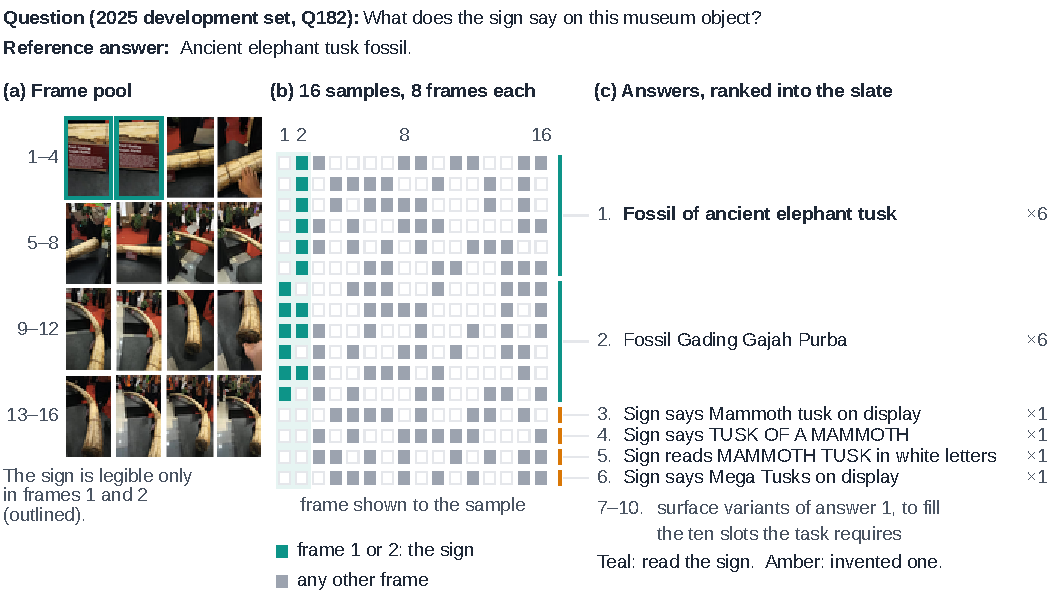
\includegraphics{figures/fig_example.pdf}
\caption{One development question through the Task~1 pipeline, recomputed from
the run's own records. (a)~The frame pool; the sign is legible only in frames 1
and 2. (b)~The eight frames each of 16 samples was shown, rows grouped by the
answer the sample gave. (c)~Those answers in slate order, with how many samples
gave each. Every sample shown frame 1 or 2 read the sign, copying it when frame
1 was among its frames and translating it when only frame 2 was; the four that
saw neither each invented a different sign. Counting repeats puts the
translation, which matches the reference, first.}
\label{fig:example}
\end{figure*}

\paragraph{Task~2.}
Each question gets three votes. A vote shows the model a random subset of 8, 12
or 16 frames (more for questions whose wording suggests text, audio or timing),
the question, a transcript when the question seems to concern audio (14\,\% of
test questions), and the options lettered in released order. The model describes
the evidence, evaluates each option and ends with a full ranking. The first vote
runs at temperature 0 and the other two at 0.7. Votes are combined by
MRR-weighted Borda count; a vote that names fewer than two options is asked again
once and otherwise dropped.

\paragraph{Two-tier escalation.}
The gold is always among the released options, so an injected option ``None of
the above can be determined from the frames shown'' can never be correct, but it
can signal doubt. Offered in the answering pass, it costs accuracy: 61.0\,\%
against a mean of 67.6\,\% for the 8B runs without it. Its flag is informative,
though: items where it fires are wrong 63\,\% of the time, against 22\,\% for the
rest. We therefore keep it out of the answers. A clean 8B pass answers. A second
8B pass with the injected option supplies features (the abstention flag, the
Borda margin between the top two options, disagreement between votes, option
count), and a logistic regression on them sends the items most likely to be wrong
to a 32B pass. We fixed this policy in writing before the 2026 run that fed it
had finished.

\subsection{Runs}
\label{sec:runs}

Every run passes the official validator on all 2,443 questions. Tables use the
short names given in parentheses.

\paragraph{Task~1, all Qwen3-VL-8B\@.}
\run{BiTeM\_cons8b\_s8}: the sampling pipeline with $S=8$.
\run{BiTeM\_cons8b\_s16}: the same with $S=16$; our flagship.
\run{BiTeM\_fewshot8b}: $S=8$ plus four 2025 examples. \run{BiTeM\_all8b}: as
\texttt{fewshot8b}, plus routed transcripts. \run{BiTeM\_v3control}: our earlier
prompt format, one call for ten answers, entered as a control we expected to be
our worst run.

\paragraph{Task~2.}
\run{BiTeM\_mc32b} (\texttt{mc\_32b\_prod}): Qwen3-VL-32B, nominated as primary.
\run{BiTeM\_mc30b} (\texttt{mc\_30b\_prod}): Qwen3-VL-30B-A3B.
\run{BiTeM\_mc122b} (\texttt{mc\_122b\_prod}): Qwen3.5-122B.
\run{BiTeM\_mc32bdense} (\texttt{mc\_32b\_dense}): \texttt{mc32b} with 32--64
frames for the 212 videos longer than 40 seconds and 16 frames per vote.
\run{BiTeM\_mcfusion} (\texttt{mc\_fusion}): reciprocal-rank fusion of the 32B,
122B and 30B option rankings. We entered \texttt{mc30b} and \texttt{mc122b} for
diversity; \texttt{mc30b} disagrees with \texttt{mc32b}'s top answer on 20\,\% of
questions. We withheld four other runs: a plain 8B run; an 8B run with partial
transcripts, which agrees with the plain one on 98\,\% of top answers and so
cannot differ from it by more than 2.1 points; the two-tier run, dropped by a
rule fixed in writing before it was built (it agreed with \texttt{mc32b} on
96.0\,\% of top answers, above our 95\,\% limit); and a hybrid of the dense and
fusion runs.

%% ==================== results
\section{Results}
\label{sec:results}

The first five subsections report development measurements on 2025 data, made
before the official scores were released. The last two use the official 2026
scores.

\subsection{How much the development set can resolve}
\label{sec:floor}

We ran one 8B configuration four times on the 497 development items, with the
same model, prompt, frames and settings. The runs differed only in inert
command-line details, the frame-sampling seed and the GPU partition that served
them, and Ollama does not seed sampling at temperature 0.7. They scored 65.6,
67.4, 67.8 and 69.6\,\% (Figure~\ref{fig:floor}a).

\begin{figure*}[t]
%% source: paper/figures/make_figures.py, which reads the data on disk and asserts
%%   that every plotted value matches the corresponding table in this paper. Drawn
%%   at final size (included unscaled) so that no text is below NIST's 9 pt minimum.
\centering
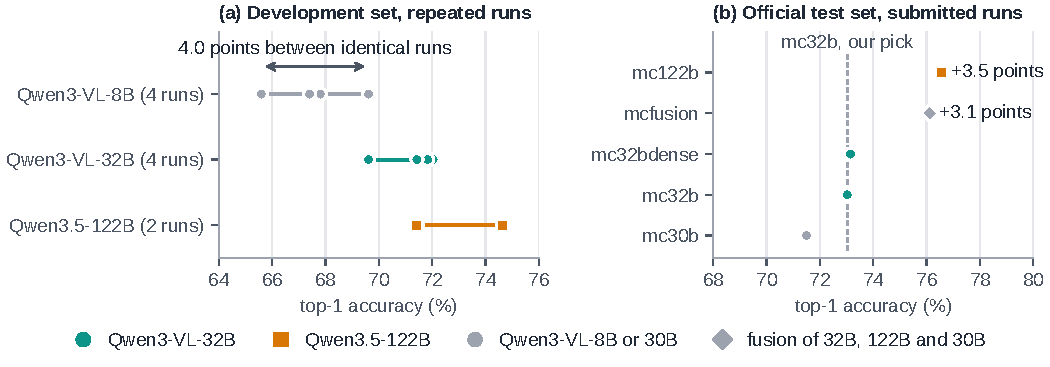
\includegraphics{figures/fig_floor.pdf}
\caption{Task~2: what the development set could and could not resolve.
(a)~Top-1 accuracy of repeated runs on the 497-item development set. The four
8B runs share one configuration and still span 4.0 points, and the 32B and 122B
ranges overlap. (b)~Official top-1 of the five submitted runs on 2,428
questions, with the difference from \texttt{mc32b}, the run we nominated as
primary. Both labelled differences are significant by exact McNemar test
($p<10^{-5}$). The panels share one scale, so the spread between identical runs
in (a) can be compared directly with the effects in (b).}
\label{fig:floor}
\end{figure*}

One of the six exact McNemar tests between pairs of these runs gives $p=0.017$.
That is not a fault of the test, which already accounts for items that flip from
run to run, and one rejection in six tests is unremarkable. The 4-point range is
not a usable threshold either, since the range of $k$ runs grows with $k$. The
informative quantity is the variance. A fifth of the items (20.7\,\%) flip
between the four runs. If flips were independent across items, run accuracy
would vary with a standard deviation of 1.07 points; the observed one is 1.65,
which implies a component of about 1.3 points shared by all items of a run. This
is the part of run-to-run variation that McNemar's test cannot see, because it
treats items as independent. With four runs the excess is suggestive, not
established (permutation test within items, $p=0.07$), and the four 32B runs show
little of it (1.10 observed against 0.98 predicted, $p=0.30$).

Comparisons between single runs inherit this variation. The same 32B run is
between 2.4 and 6.4 points above the four 8B runs, depending on which replicate
is the baseline, and its McNemar $p$ ranges from 0.19 to 0.0002. Pooling each
item's replicates gives the comparisons the set can support. Four 32B runs beat
four 8B runs by 3.6 points (sign-flip permutation over items, $p=0.006$; adding
the shared run-level component estimated above leaves $p\approx0.01$). Two
Qwen3.5-122B runs beat the four 32B runs by 1.8 points ($p=0.16$), a difference
the set cannot separate from zero; the official set later put it at 3.5 points
($p<10^{-5}$, Section~\ref{sec:official}). At the discordance between our
replicates, 497 items give 80\,\% power only to differences of about 4.3 points.
An oracle that counts an item as solved when any of the four 8B runs is right
scores 78.1\,\%, 10.5 points above their mean, so much of the apparent
complementarity between our runs is the same flipping counted several times.

\subsection{What the multiple-choice labels are made of}
\label{sec:benchmark}

\paragraph{MC is AG with distractors.}
In the 2025 collection, every MC gold option is identical to the AG reference
for its question, in all 1,996 items that have both. There is one reference per
question and a constant relevance grade. The two tasks therefore share their
annotation errors: a wrong reference costs points on Task~1 and becomes the
correct option on Task~2, and tuning on one task while reporting on the other is
not cross-validation.

\paragraph{Non-answers and contested items.}
Six references are non-answers (``I don't know.'' four times, ``Nothing.'' and
``None.''), and all six became MC golds. Q40 asks which chemical is being mixed
and keys ``I don't know.'' over ``Sodium bicarbonate.'', so a system that names
the chemical is wrong on both tasks. Reading 22 contested items, we also found
keys with several true options, golds the video does not support, factually
wrong golds, and questions with a false premise (Q135 asks about a woman in pink,
and there is none). These items were chosen for being contested, so they do not
estimate a defect rate.

\paragraph{The option-length artifact.}
Choosing the longest option, without the video or the question, is correct on
47.1\,\% of the 2025 four-option questions, against 25\,\% chance
(Figure~\ref{fig:length}). The effect depends on the question type. It is
strongest for \emph{how}, \emph{why} and \emph{what} questions (54 to 63\,\%),
where the gold is a sentence written while watching and the distractors were
written afterwards to be wrong. It disappears or reverses for counting and yes/no
questions, whose answer space is closed. On the released 2026 labels the same
rule is correct on 40.9\,\% of questions. Corrected for chance, as
$(\mathrm{acc}-\mathrm{chance})/(1-\mathrm{chance})$, that is 0.30, against 0.29
in 2025, and on four-option items it is 49.2\,\% against 47.1\,\%: the artifact
has not weakened. Our best 2025 development score, 74.8\,\%, is 28 points above
this baseline.

\begin{figure}[t]
%% source: paper/figures/make_figures.py; drawn at final size, included unscaled (no text below 9 pt).
%% source: re-derived 2026-09-15 from data/vqa/topics/mc_topics_2025.csv with
%%   golds resolved through data/vqa/qrels_mc.csv, options stripped and the first
%%   option of maximal character length taken (eval/vqa/eval_mc.py's own baseline
%%   convention), official 18-item SKIP set applied -> 931/1978 = 47.07%.
%% TYPE RULE, stated because three incompatible rules are in play across this
%%   project's notes and they disagree by up to 46 items on *what*. Applied to the
%%   question text of mc_topics_2025.csv (field 3), lowercased, in this order:
%%   (1) counting  if /how many|how much|number of/ matches anywhere;
%%   (2) yes/no    if the string STARTS with is|are|does|do|did|was|were|can|
%%                 could|will|would|has|have|had as a whole word;
%%   (3) otherwise the earliest-occurring whole word among
%%                 {what, why, how, where, when, who, which};
%%   (4) otherwise other.
%%   Full partition, n and longest==gold: what 1324 54.15%, counting 243 16.87%,
%%   why 181 55.80%, yes/no 89 12.36%, how 48 62.50%, who 27 25.93%,
%%   where 24 45.83%, when 20 45.00%, other 12 25.00%, which 10 10.00%.
%%   1324+243+181+89+48+27+24+20+12+10 = 1978; hits 717+41+101+11+30+7+11+9+3+1 = 931.
%%   (Corrected 2026-11-09: this comment read "why 181 56.35%"; its own hit count,
%%   101/181, is 55.80%, which is what the former table printed.)
\centering
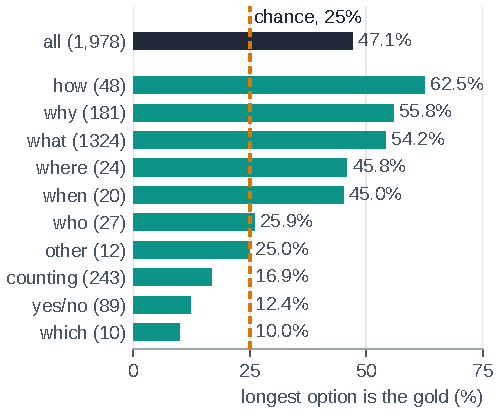
\includegraphics{figures/fig_length.pdf}
\caption{How often the longest option is the gold, by question type, on the 2025
multiple-choice set ($n=1978$, four options, chance 25\,\%). Counts in
parentheses. A question is \emph{counting} if it asks how many or how much,
\emph{yes/no} if it starts with an auxiliary verb, and otherwise takes its first
\emph{wh}-word.}
\label{fig:length}
\end{figure}

\paragraph{Unreachable golds.}
Four 2025 golds (Q332, Q387, Q596, Q1745) do not appear among their own options,
so no run could score them. The AG topics file puts a space before each opening
quote, which breaks CSV quoting~\cite{rfc4180} and splits 41 rows at internal
commas; in three of them the split reaches the answer column. Q332 has a missing
quote in the MC file. Together with the 18 questions whose videos were
unavailable, which the 2025 scorer skips but keeps in its denominator, these cap
the official 2025 MC score at 98.9\,\%. A five-line check (each row parses to its
declared fields, and each gold appears among its options) names all four before
release.

\subsection{Development ablations}
\label{sec:negatives}

Table~\ref{tab:summary} lists every MC effect we measured on development data,
and Figure~\ref{fig:forest} plots the whole-set ones against the range of the
four identical runs. Besides model size (Section~\ref{sec:floor}), two effects
are clearly larger than run-to-run variation, and both act on a subset of
questions.

\begin{table*}[t]
\caption{Every MC accuracy effect we measured on development data: difference in
top-1 accuracy (points) and exact McNemar $p$. The first row compares the best and
worst of four identical 8B runs; rows with $n<497$ are question subsets. $^{\dagger}$Each item's replicate runs pooled;
sign-flip permutation test over items. Router comparisons are in
Figure~\ref{fig:router}.}
\label{tab:summary}
\small
\begin{tabular}{lrrr}
\toprule
effect & $n$ & $\Delta$ & $p$ \\
\midrule
\emph{identical configuration, best vs worst run} & 497 & 4.02 & 0.0169 \\
32B vs 8B, four runs each$^{\dagger}$ & 497 & $+3.62$ & 0.006 \\
122B vs 32B, two vs four runs$^{\dagger}$ & 497 & $+1.81$ & 0.16 \\
30B-A3B vs 8B & 497 & $+2.41$ & 0.2354 \\
32B vs 30B-A3B & 497 & $+2.21$ & 0.2480 \\
transcripts and larger frame budget, 32B & 497 & $+2.62$ & 0.0660 \\
\textbf{transcripts, injected items} & \textbf{48} & $\mathbf{+20.83}$ & \textbf{0.0129} \\
broadcast vs routed, 32B & 497 & $+0.00$ & 1.00 \\
re-asking unparsable votes & 497 & $+0.20$ & 1.00 \\
16 vs 8 frames, temporal & 120 & $+0.00$ & 1.00 \\
12 vs 8 frames, temporal & 120 & $+2.50$ & 0.5488 \\
16 vs 8 frames, audio & 120 & $-0.83$ & 1.00 \\
16 frames $+$ ASR, audio & 120 & $+10.00$ & 0.0118 \\
best rank fusion vs best single run & 497 & $+0.80$ & n/a \\
\textbf{oracle vs best single run} & 497 & $\mathbf{+12.47}$ & n/a \\
\bottomrule
\end{tabular}
\end{table*}
\begin{figure}[t]
%% source: paper/figures/make_figures.py; drawn at final size, included unscaled (no text below 9 pt).
%%   Plots the 497-item rows of Table tab:summary; the script asserts each value is in it.
\centering
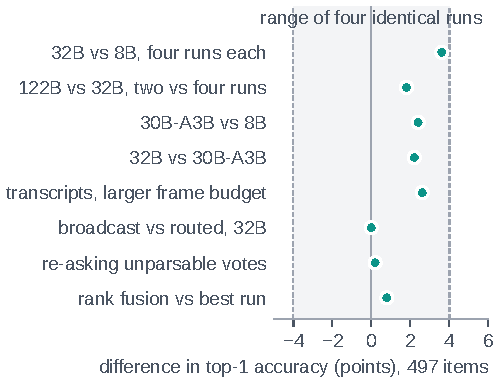
\includegraphics{figures/fig_forest.pdf}
\caption{Whole-set development effects from Table~\ref{tab:summary}. Shaded: the
range between four identical 8B runs, shown for scale and not as a significance
threshold. The oracle ($+12.5$ points) is off the scale.}
\label{fig:forest}
\end{figure}

\paragraph{Transcripts.}
On the 48 development questions that receive a transcript, 32B accuracy rises
from 52.1 to 72.9\,\% ($p=0.013$), which is 10 more correct answers, or 2.0 points over all 497
items. The whole-set comparison shows 2.6 points because its transcript runs
also used a larger frame budget. Routing transcripts only to questions about speech scored the same as
giving one to every question that has one (74.65\,\% both, 14 discordant items
each way), so we kept routing because it is cheaper. Sixteen frames with a
transcript beat eight frames without one by 10 points on the audio slice
($p=0.012$), two thirds of it from the transcript.

\paragraph{Frames.}
Sixteen frames instead of eight changed nothing on the temporal or audio slices
($+0.0$ and $-0.8$ points, 120 items each). No development video is longer than
30 seconds, while a fifth of the test questions come from clips of up to 389, so
this says nothing about long videos; the dense run tests them
(Section~\ref{sec:official}).

\paragraph{Fusion and parsing.}
Over seven development runs, an oracle that counts an item as solved when any run
ranks the gold first scores 87.1\,\%, against 74.7\,\% for the best single run.
The best combiner we found, a reciprocal-rank sum, recovers 0.8 of those 12.5
points; the rest is mostly the flipping measured above. Asking a failed vote
again lowered the share of questions where no vote parsed, and the released order
was emitted, from 28 to 25 of 497. A blind human rater scored 11 of 15 contested
items, as did our 32B run.

\subsection{Model size and escalation}
\label{sec:cascaderes}

Per question, the 8B model took 11.8 seconds and the 32B model 35.2 on our shared
GPUs, so 32B's 3.6-point gain costs three times the time. We fitted the
escalation policy on 1,822 eight-option development items with five-fold
cross-validation (Figure~\ref{fig:router}). Both policies choose which items to
escalate better than chance. At a 50\,\% budget the learned router gains 1.9
points over escalating the same number of items at random, about four standard
deviations of the random draw. A single feature, the Borda margin, gains up to
1.7 points, at a 30\,\% budget.

\begin{figure}[t]
%% source: paper/figures/make_figures.py; drawn at final size, included unscaled (no text below 9 pt).
%% source: logs/router_analysis.txt, written by
%%   scripts/run_router_analysis.sh -> eval/vqa/router_analysis.py with
%%   --votes /tmp/rt8_{0,1,2}.jsonl (copied to data/vqa/2026/evidence/rt8_*.jsonl)
%%   --tier1 /tmp/e7_{turbo,largev3}.csv --tier2 the merged e5_32b_{notr,tr} arms.
%%   The escalation budget was fixed in advance in
%%   data/vqa/2026/evidence/ROUTER_PREREG.md, before the 2026 signal run finished.
\centering
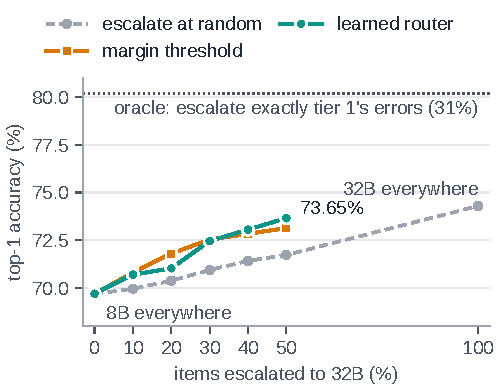
\includegraphics{figures/fig_router.pdf}
\caption{Two-tier escalation on $n=1822$ development items, five-fold
cross-validated: top-1 accuracy against the share of items escalated from 8B to
32B. Both routing policies beat escalating the same number of items at random. At
a 50\,\% budget the learned router reaches 73.65\,\%, against 74.29\,\% for 32B
on every item and 71.72\,\% for random escalation.}
\label{fig:router}
\end{figure}

Neither beats running 32B on every item (74.3\,\%), and the cost of the second 8B
pass makes routing worse than it looks. At a 50\,\% budget the learned router
costs about 41 seconds per question (two 8B passes and half a 32B pass) against
35 for 32B everywhere, and it is less accurate (73.7 against 74.3\,\%). The
answering pass computes the same Borda tally as the second pass, so a margin
router reading it would need no second pass and cost about 22 seconds per question at a 30\,\% budget, where the margin router
scored 72.5\,\% (against 74.3\,\% for 32B everywhere at 35 seconds); we measured
the margin only on the second pass. An
oracle that escalates exactly the 8B errors (31\,\% of items) would reach
80.2\,\%. An escalation rule chosen by hand on the 497 items, which appeared to
match 32B at 16\,\% of the budget, did not survive cross-validation on the
larger set.

\subsection{Candidate selection}
\label{sec:selection}

For Task~1, no selection rule we tried at 16 samples (a vision-language verifier,
cluster mass, centrality, length priors) beat ranking answers by how often they
recur. The run that topped Task~1, \texttt{NII\_UIT-mbr128}, has a name that suggests minimum-Bayes-risk (MBR) selection over 128 samples
(their paper is not yet out), so we tested MBR across sample budgets. We drew 128 samples for each of 300 development topics, took the
smaller budgets as prefixes of the same pool, and compared rules per topic on
identical candidates. We fixed the main comparison in writing before the pool had
finished generating.

\begin{figure}[t]
%% source: paper/figures/make_figures.py, which reads the data on disk and asserts
%%   that every plotted value matches the corresponding table in this paper. Drawn
%%   at final size (included unscaled) so that no text is below NIST's 9 pt minimum.
\centering
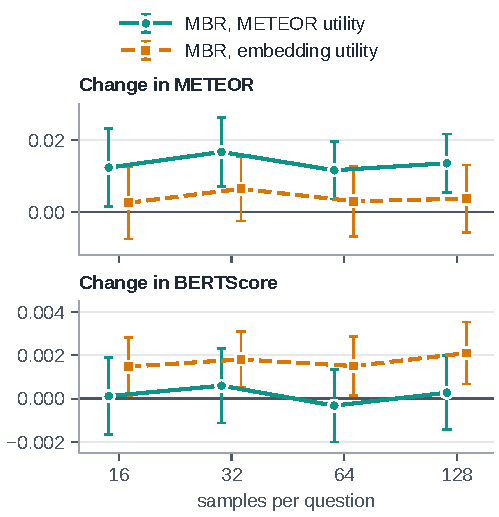
\includegraphics{figures/fig_mbr.pdf}
\caption{Minimum-Bayes-risk selection against repeat-counting, by sample budget,
on 300 development topics: mean paired difference, with error bars of two
standard errors. Each rule moves the measure that is its own utility, METEOR
for the METEOR utility and BERTScore for the embedding utility, and leaves the
other where it was. Neither gain changes measurably with the budget.}
\label{fig:mbr}
\end{figure}

MBR with a METEOR utility beats repeat-counting by 0.014 METEOR at 128 samples
(3.3 standard errors), and by a similar margin at every budget, but leaves
BERTScore unchanged. MBR with an embedding utility does the opposite
(Figure~\ref{fig:mbr}). Each rule improves the measure it optimises and no other,
so it decides which measure to favour, not which answer is better. The gain does
not grow with the budget (0.012 at 16 samples, 0.014 at 128), and at best it
closes 9\,\% of our METEOR gap to the leader. Repeat-counting itself beats a
random pick from the same pool by about 0.01 METEOR. The gap to an oracle that
knows the reference grows from 0.08 to 0.13 METEOR with the budget while every
rule stays flat, which is what a maximum over more noisy draws does on its own.

\subsection{Official scores}
\label{sec:official}

Our best runs placed 7th of 15 teams on Task~1, where the leader scored 0.511
STS@1, and 10th of 13 on Task~2, where the leader scored 84.8\,\%.
Tables~\ref{tab:runs} and~\ref{tab:ag} give our scores.

\begin{table*}[t]
\caption{The five Task~2 runs submitted, with official 2026 scores
(released 2026-09-28; $n=2428$ after NIST excluded 15 queries field-wide).
Development figures are the estimates available when the runs were chosen.
The two rightmost columns give the official accuracy and the difference from
the run we had nominated as primary, with its McNemar test.}
%% source: submissions/vqa2026/BiTeM_mc_*.json, six files, each 2443 entries whose
%%   answer lists are exact permutations of the released Task2_v2 options.
%%   Dev evidence from data/vqa/2026/evidence/ as above; top-1 disagreement
%%   re-derived 2026-09-15 across the built run JSONs: 32b/30b 494 = 20.2%,
%%   32b/8b 642 = 26.3%, 8b/8b_asr 51 = 2.1%.
%%   Official top-1 and the McNemar columns: submissions/vqa2026/official_results/.
\label{tab:runs}
\small
\begin{tabular}{llrr}
\toprule
Task 2 run (model) & dev evidence & official top-1 & vs.\ 32B \\
\midrule
\texttt{mc\_122b\_prod} (122B) & 74.65 / 71.43\,\%, ``ties 32B'' & \textbf{76.57\,\%} & $+3.54$, $p<10^{-5}$ \\
\texttt{mc\_fusion} (32B+122B+30B) & not built when written & 76.11\,\% & $+3.09$, $p<10^{-5}$ \\
\texttt{mc\_32b\_dense} (32B)  & none possible (long clips) & 73.15\,\% & $+0.12$, $p=0.89$ \\
\texttt{mc\_32b\_prod} (32B)   & 72.03\,\%, our pick & 73.02\,\% & n/a \\
\texttt{mc\_30b\_prod} (30B)   & 69.82\,\%; 20.2\,\% $\neq$ 32B & 71.50\,\% & $-1.52$, $p=0.051$ \\
\bottomrule
\end{tabular}
\end{table*}


\paragraph{Task~2: prediction and outcome.}
We nominated \texttt{mc32b} as primary, and it finished fourth of our five. We
entered \texttt{mc122b} for diversity and expected a tie with 32B. It is our best
run, 3.5 points above \texttt{mc32b} (exact McNemar, $p<10^{-5}$). We nearly left
out fusion, which was only 0.8 points above our best single run on development
data. It scored 76.1\,\%, 3.1 points above \texttt{mc32b} ($p<10^{-5}$), level
with \texttt{mc122b} ($p=0.46$), and has our highest MRR (0.851). Both effects are
about as large as the range of our identical development runs
(Figure~\ref{fig:floor}), and at the official discordance the 497-item set had
only 54\,\% power to detect them. \texttt{mc30b} scored 1.5 points below
\texttt{mc32b} ($p=0.051$). The dense run, which gave 32 to 64 frames to the 212
test videos longer than 40 seconds, scored 0.1 points above \texttt{mc32b}
($p=0.89$) for 78 GPU-hours; on long clips as well, more frames did not help the
32B model.

\begin{table}[t]
\caption{Official Task~1 scores, human-answer-only reference mode, $n=2428$.
\texttt{v3control} is the control we expected to be our worst run.}
\label{tab:ag}
\footnotesize
\setlength{\tabcolsep}{4pt}
\begin{tabular}{lrrrr}
\toprule
Task 1 run & STS@1 & MET@1 & BERT@1 & MET nDCG \\
\midrule
\texttt{cons8b\_s16} & \textbf{0.4605} & 0.1696 & 0.8831 & 0.7538 \\
\texttt{all8b}       & 0.4595 & 0.1878 & \textbf{0.8858} & 0.7804 \\
\texttt{cons8b\_s8}  & 0.4592 & 0.1693 & 0.8830 & 0.7580 \\
\texttt{fewshot8b}   & 0.4553 & 0.1812 & 0.8849 & 0.7766 \\
\texttt{v3control}   & 0.4321 & \textbf{0.2238} & 0.8689 & \textbf{0.8569} \\
\bottomrule
\end{tabular}
\end{table}
\begin{figure}[t]
%% source: paper/figures/make_figures.py, which reads the data on disk and asserts
%%   that every plotted value matches the corresponding table in this paper. Drawn
%%   at final size (included unscaled) so that no text is below NIST's 9 pt minimum.
\centering
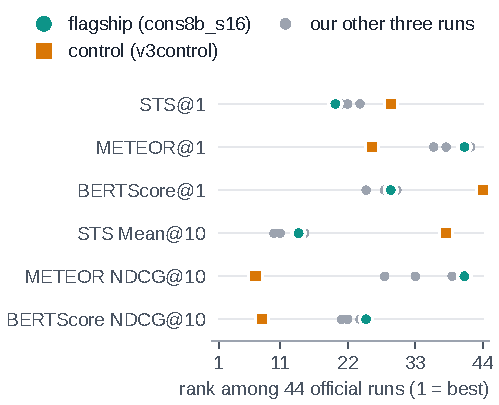
\includegraphics{figures/fig_ranks.pdf}
\caption{Rank of our five Task~1 runs among the 44 official runs under six
official measures (human-answer-only references). The flagship is 14th on the
mean over ten answers it was built for and 41st on METEOR NDCG@10; the
deliberate control is last on BERTScore@1 and 7th on METEOR NDCG@10.}
\label{fig:ranks}
\end{figure}

\paragraph{Task~1: the measures disagree.}
The control, which uses our earlier prompt format and was expected to be our
worst run, is last of our five on STS@1, 0.023 below the next run, but first on
METEOR@1 (0.036 above the next) and on METEOR NDCG@10 (0.077 above the next).
Our flagship ranks 14th of the 44 official runs on mean STS over ten answers, the
measure it was built for, but 20th on STS@1 and 41st on METEOR NDCG@10
(Figure~\ref{fig:ranks}). METEOR weights recall nine to one, so it rewards the
long, speculative answers that a mean over ten answers penalises.

\subsection{Post-submission analysis}
\label{sec:posthoc}

NIST returned per-query results, with the gold option for each scored Task~2
question and the official score of every answer in our Task~1 runs. From them we
reproduce every official number in Tables~\ref{tab:runs} and~\ref{tab:ag} to six
decimals, so any slate or combination built from our answers can be scored as
NIST would score it. The rules below were written after the scores were released,
and we report the best of each family.

\begin{table*}[t]
\caption{Task~1 under the official measures (MET is METEOR, BERT is BERTScore F1),
scored against the human reference only. Submitted runs and the field leader carry NIST's values. The constructed
rows reuse answers we submitted and are scored from NIST's per-answer scores,
except that the nonsense strings, which METEOR scores at zero, have no BERTScore
or STS we can know. Parentheses give the rank among the 44 official runs, with a
constructed row ranked as if it replaced the run it is built from.}
\label{tab:metricbias}
\footnotesize
\setlength{\tabcolsep}{4pt}
\begin{tabular}{lrrrrrr}
\toprule
slate & STS@1 & MET@1 & BERT@1 & STS Mean@10 & MET NDCG@10 & BERT NDCG@10 \\
\midrule
flagship \texttt{cons8b\_s16} & 0.4605 (20) & 0.1696 (41) & 0.8831 (29) & 0.4473 (14) & 0.7538 (41) & 0.9952 (25) \\
control \texttt{v3control} & 0.4321 (29) & 0.2238 (26) & 0.8689 (44) & 0.3676 (38) & 0.8569 (7) & 0.9972 (8) \\
flagship 1st, control 2nd--10th & 0.4605 (20) & 0.1696 (41) & 0.8831 (29) & 0.3794 (31) & 0.8110 (23) & 0.9967 (12) \\
flagship 1st, nine nonsense & 0.4605 (20) & 0.1696 (41) & 0.8831 (29) & n/a & 0.7492 (42) & n/a \\
control 1st, nine nonsense & 0.4321 (29) & 0.2238 (26) & 0.8689 (44) & n/a & 0.9024 (1) & n/a \\
\midrule
leader \texttt{NII\_UIT-mbr128} & 0.5112 (1) & 0.2975 (1) & 0.8969 (5) & 0.4620 (2) & 0.8813 (1) & 0.9980 (3) \\
\bottomrule
\end{tabular}
\end{table*}

\paragraph{What METEOR rewards.}
METEOR is zero for an answer that shares no word with the reference, and the
share of zeros falls from 35\,\% of answers of one or two words to 13\,\% at
eight to twelve. Our flagship's first answers average 5.7 words against 14.6 for
the control, and 25\,\% of them score zero on METEOR@1, against 10\,\% for the
control. At matched length the two runs score alike. The zero-METEOR answers are
not all good answers, though: their mean STS is 0.32, against 0.51 for the
flagship's other first answers.

\paragraph{The within-slate NDCG can be gamed.}
NDCG@10 takes its ideal order from the slate's own gains, so a slate scores 1
whenever its order matches its own scores, whatever their level. A first answer
that scores, followed by nine that score nothing, reaches 1.0. The control's first answers followed by nine nonsense strings would score 0.902
on METEOR NDCG@10 (Table~\ref{tab:metricbias}), above every official run (the best is 0.881).

\paragraph{Trading one measure for another.}
Keeping the flagship's first answer and filling the slate with the control's
next nine answers leaves every @1 score unchanged (Table~\ref{tab:metricbias}). It lifts METEOR NDCG@10 from
41st to 23rd and BERTScore NDCG@10 from 25th to 12th (both $p<0.002$,
Holm-adjusted), and drops mean STS over ten answers from 14th to 31st. No rule we
tried improved STS@1, including MBR with a token-overlap utility over our
submitted answers (changes between $-0.010$ and $+0.004$, none significant), as
Section~\ref{sec:selection} predicts for a utility that is not the measure. Our
flagship's STS@1 is 0.110 below the best of its own ten answers, against 0.047
for the leader, so the first answer is where we lose most.

\paragraph{Punctuation changes STS\@.}
The surface variants we used to fill slots received a different official STS
from the answer they copy in all but 51 of 50,771 cases, 0.013 lower on average.
Adding a full stop to ``The bride and groom vanish into mist'' lowers its STS
from 0.332 to 0.298.

\paragraph{Task~2.}
No label-free combination of our runs beats \texttt{mc122b} significantly (the
best gains 0.25 points, $p=0.62$), although an oracle over our nine runs would
reach 86.6\,\%. The four runs we withheld would have scored 74.9\,\% (hybrid),
72.9\,\% (two-tier) and 67.4 and 66.6\,\% (the 8B runs). The 122B model's lead
over 32B is larger on the 479 long-clip questions (63.3 against 56.6\,\%) than on
the rest (79.8 against 77.1\,\%).

\paragraph{How many development items we needed.}
At the official discordance between \texttt{mc122b} and \texttt{mc32b} (13\,\% of
questions), an exact McNemar test has about 54\,\% power at 497 items, 80\,\% at
about 880, and 98\,\% at the 1,822 items we already used for the router. One 122B
pass over 1,822 items takes about 22 hours, less than the dense run cost.

%% ==================== discussion
\section{Discussion and Conclusions}

\subsection{Findings for the organisers}

Several of our findings concern the benchmark and the scorer, not our system.
Table~\ref{tab:organisers} lists them with a suggested fix for each. Most can be
detected from the released files before any system is run.

\begin{table*}[t]
\caption{Issues in the benchmark and scorer that affect every team, with evidence
and a suggested fix. The year in parentheses is the collection or scorer in which
we measured the issue.}
\label{tab:organisers}
\small
\setlength{\tabcolsep}{4pt}
\begin{tabular}{>{\raggedright\arraybackslash}p{0.21\textwidth}>{\raggedright\arraybackslash}p{0.43\textwidth}>{\raggedright\arraybackslash}p{0.29\textwidth}}
\toprule
issue & evidence & suggested fix \\
\midrule
MC gold copied from AG & identical to the AG reference in 1,996 of 1,996 items; one reference per question, no adjudication (2025) & an independent MC key, or several references per question \\
Non-answer golds & six references such as ``I don't know.'' became MC golds (2025) & reject non-answers with a lexicon check before release \\
Unreachable golds & four golds absent from their own options, from CSV quoting errors (2025) & check that each gold appears among its options; quote per RFC~4180 \\
Skipped questions in the denominator & 18 questions without a video counted as wrong for every team (2025 scorer; the 2026 scores exclude them) & divide by the questions actually scored \\
Option length & the longest option is the gold on 47\,\% of questions against 25\,\% chance (2025) and on 41\,\% against 15\,\% (2026); 0.29 and 0.30 after correcting for chance & publish the longest-option baseline next to chance; balance option lengths \\
Shell call in the AG scorer & answers reach Perl unescaped: \texttt{\&} and \texttt{\#} truncate an answer, and non-ASCII text scores 0 (2025 scorer) & pass answers through a file, or escape them \\
STS depends on punctuation & a full stop moves STS from 0.332 to 0.298; slot-filling variants score differently from their source in 50,720 of 50,771 cases (2026) & normalise punctuation before scoring \\
STS needs a 2013 web service & unreachable since about 12 August 2026, so no team could score STS locally & ship a local STS model with the scorer \\
Within-slate NDCG can be gamed & one real answer plus nine nonsense strings scores 0.902 on METEOR NDCG@10, above every official run (0.881) (2026) & normalise by a fixed ideal slate, not by the slate's own gains \\
\bottomrule
\end{tabular}
\end{table*}

\subsection{What we would do differently}

We would run the baseline several times before comparing anything, and compare
configurations by pooling replicates per item. We would size the development set
for the effects we care about: about 1,200 items to detect 3 points at the
disagreement rate we saw between models. We would never take
development data as a contiguous slice of the topic file, since file order
follows collection batch and annotation session. We would make every component
report a counter for what it does: three of our nulls came from components that
were not running (a transcript that never reached the model, a translation flag
the speech model ignores, a draft stage computed and discarded). And we would
test the scorer. Ours stripped quote characters the CSV reader had already
removed, which made the golds of 14 development and 22 test questions
unmatchable until we fixed it. Some engineering pitfalls cost us time:
\begin{itemize}\setlength{\itemsep}{1pt}
\item Ollama reserves about 48\,GB of KV cache unless \texttt{num\_ctx} is set,
and the 8B model then does not fit on a 20\,GB GPU slice.
\item faster-whisper's default voice-activity filter returns empty transcripts
on sung vocals; we disabled it.
\item large-v3-turbo accepts \texttt{--task translate} and ignores it: 40\,\% of
non-empty development transcripts came back in a non-Latin script, and a quarter
of the 2026 videos are not in English.
\item When a model names only some options, the parser appends the rest in
released order; a vote naming fewer than two options is pure padding.
\end{itemize}

\subsection{Limitations}

Our MC development set is our own construction and differs from the 2026 items,
most of all in how similar the options are, so it ranks systems but does not
predict accuracy. No labelled data we hold covers long videos. The official STS
calls a 2013 web service that has not answered since about 12 August 2026, so our
development STS figures predate that date and we could not score STS locally
after it. Code, our development-set runs and the analysis and figure scripts are at
\url{https://github.com/ecsltae/trecvid2026-vqa}.

\subsection{Conclusions}

On 497 development items, runs of one configuration spread over 4 points, and
two 3-point effects we dismissed there were real on the official set. The
multiple-choice gold is the free-text reference copied, the longest option is
still correct far above chance in 2026, and the answer-generation measures rank
the same run anywhere from 14th to 41st of 44. For our own work, a development set of about 1,200 items and several replicates per configuration
would have let us nominate the right primary run.

\bibliographystyle{ACM-Reference-Format}
\bibliography{refs}

\end{document}
